\documentclass[conference]{IEEEtran}
\IEEEoverridecommandlockouts

\usepackage{graphicx}
\usepackage{amsmath,amssymb,amsfonts}
\usepackage{algorithmic}
\usepackage{textcomp}
\usepackage{booktabs}
\usepackage{multirow}
\usepackage{hyperref}
\usepackage{xcolor}
\usepackage{subcaption}
\usepackage{array}

\title{An Empirical Comparison of Deep Learning Architectures for Vessel ETA Prediction on Trans-Pacific Routes}

\author{
\IEEEauthorblockN{Anonymous}
\IEEEauthorblockA{Anonymous Affiliation}
}

\begin{document}

\maketitle

\begin{abstract}
Accurate Estimated Time of Arrival (ETA) prediction for ocean-going vessels is critical for port logistics, berth scheduling, and supply chain management.
While numerous deep learning architectures have been proposed for time-series forecasting, the relative effectiveness of different model families for vessel ETA prediction remains unclear, as prior studies typically evaluate only one or two architectures.
In this paper, we present a systematic empirical comparison of ten forecasting models spanning five architectural families---recurrent (LSTM, GRU), convolutional (1D-CNN, TCN), attention-based (Vanilla Transformer, Conv-Transformer, Informer), tree-based (XGBoost), and feedforward (MLP, Ridge)---on a large-scale trans-Pacific AIS dataset comprising 35.9 million position reports and 9,087 voyages.
All models are evaluated under identical data splits, feature sets, normalization, and training protocols to ensure a fair comparison.
Our results reveal that XGBoost achieves the best performance (MAE = 15.14\,h), followed closely by MLP and LSTM, while attention-based models---including the Informer---do not outperform simpler alternatives despite significantly higher parameter counts.
We further demonstrate that incorporating meteorological features yields a 7.1\% MAE reduction across architectures, and that asymmetric loss functions intended to reduce underestimation degrade overall accuracy.
These findings suggest that for single-step vessel ETA prediction, feature engineering quality---particularly distance-to-destination---dominates model architecture choice.
\end{abstract}

\section{Introduction}

Vessel Estimated Time of Arrival (ETA) prediction is a fundamental task in maritime logistics.
Accurate ETAs enable port operators to optimize berth allocation, coordinate crane assignments, and reduce vessel waiting times, with significant economic and environmental implications~\cite{unctad2023}.
The proliferation of Automatic Identification System (AIS) data---broadcasting vessel position, speed, and course at frequent intervals---has created an opportunity for data-driven approaches to ETA prediction~\cite{fang2022}.

Recent years have seen a wide range of machine learning methods applied to this problem.
Recurrent neural networks such as LSTM~\cite{zhang2022lstm} and GRU~\cite{han2021gru} naturally model the sequential nature of vessel trajectories.
Convolutional approaches, including Temporal Convolutional Networks (TCN)~\cite{bai2018tcn}, capture local temporal patterns through dilated causal convolutions.
Transformer-based architectures~\cite{dong2023transformer, zhou2021informer} leverage self-attention to model long-range dependencies.
Meanwhile, gradient-boosted tree methods like XGBoost~\cite{chen2016xgboost} remain strong competitors through hand-crafted feature engineering.

Despite this diversity of approaches, a systematic comparison under controlled conditions is lacking.
Most existing studies evaluate only one or two architectures, use different datasets with varying preprocessing pipelines, and often omit critical experimental details---making cross-paper comparisons unreliable.
Recent comprehensive surveys in time-series forecasting~\cite{kim2025comprehensive, zeng2023transformers} have emphasized the importance of fair benchmarking, revealing that simpler models often rival or surpass complex architectures when evaluated properly.

% Identify the gap
This paper addresses this gap by conducting a rigorous empirical comparison of ten forecasting models from five architectural families on a large-scale trans-Pacific AIS dataset.
Our model selection follows the taxonomy proposed by recent deep time-series forecasting surveys~\cite{kim2025comprehensive}: we include at least one representative from each major family (recurrent, convolutional, attention-based, tree-based, and feedforward) to ensure comprehensive coverage.
All models are trained and evaluated under identical conditions---same data splits, feature sets, normalization, loss function, optimizer, and early-stopping criteria---to isolate the effect of model architecture.

Our main contributions are:
\begin{enumerate}
    \item A fair, large-scale empirical comparison of ten models spanning five architectural families for vessel ETA prediction, revealing that XGBoost outperforms all neural sequence models.
    \item An analysis of the impact of meteorological feature integration, demonstrating a consistent 7.1\% MAE improvement.
    \item An investigation of asymmetric loss functions for reducing ETA underestimation, yielding a negative result that cautions against naive application of such losses.
    \item A decoupled prediction architecture that separately models sailing time and port-dwell time, reflecting their distinct underlying dynamics.
\end{enumerate}

\section{Methodology}

\subsection{Problem Formulation}

Given a vessel's historical AIS trajectory $\mathbf{X} = \{x_1, x_2, \ldots, x_T\}$, where each observation $x_t \in \mathbb{R}^{d}$ contains $d$-dimensional navigation and meteorological features at time step $t$, the objective is to predict the remaining sailing time $\hat{y} \in \mathbb{R}^{+}$ until the vessel reaches its destination port.

We decompose the total ETA into two components:
\begin{equation}
    \text{ETA}_{\text{total}} = \hat{y}_{\text{sail}} + \hat{y}_{\text{port}}
    \label{eq:decomposition}
\end{equation}
where $\hat{y}_{\text{sail}}$ denotes the predicted open-sea sailing time and $\hat{y}_{\text{port}}$ denotes the predicted port-dwell time.
This decomposition is motivated by the observation that sailing dynamics (governed by vessel speed, currents, and weather) and port operations (governed by berth availability, cargo handling, and congestion) are driven by fundamentally different factors.

\subsection{System Architecture}

The prediction system consists of three stages, as illustrated in Fig.~\ref{fig:architecture}:

\begin{enumerate}
    \item \textbf{Data Preprocessing}: Raw AIS records are cleaned, segmented into individual voyages via speed-based port-stop detection, augmented with meteorological features, and organized into fixed-length input sequences.
    \item \textbf{Sailing Time Prediction}: One of ten candidate models processes the input sequences to predict the remaining sailing time.
    \item \textbf{Port Dwell Prediction}: A separate MLP model estimates the expected port-dwell time based on destination region, arrival timing, and location features.
\end{enumerate}

\begin{figure}[t]
    \centering
    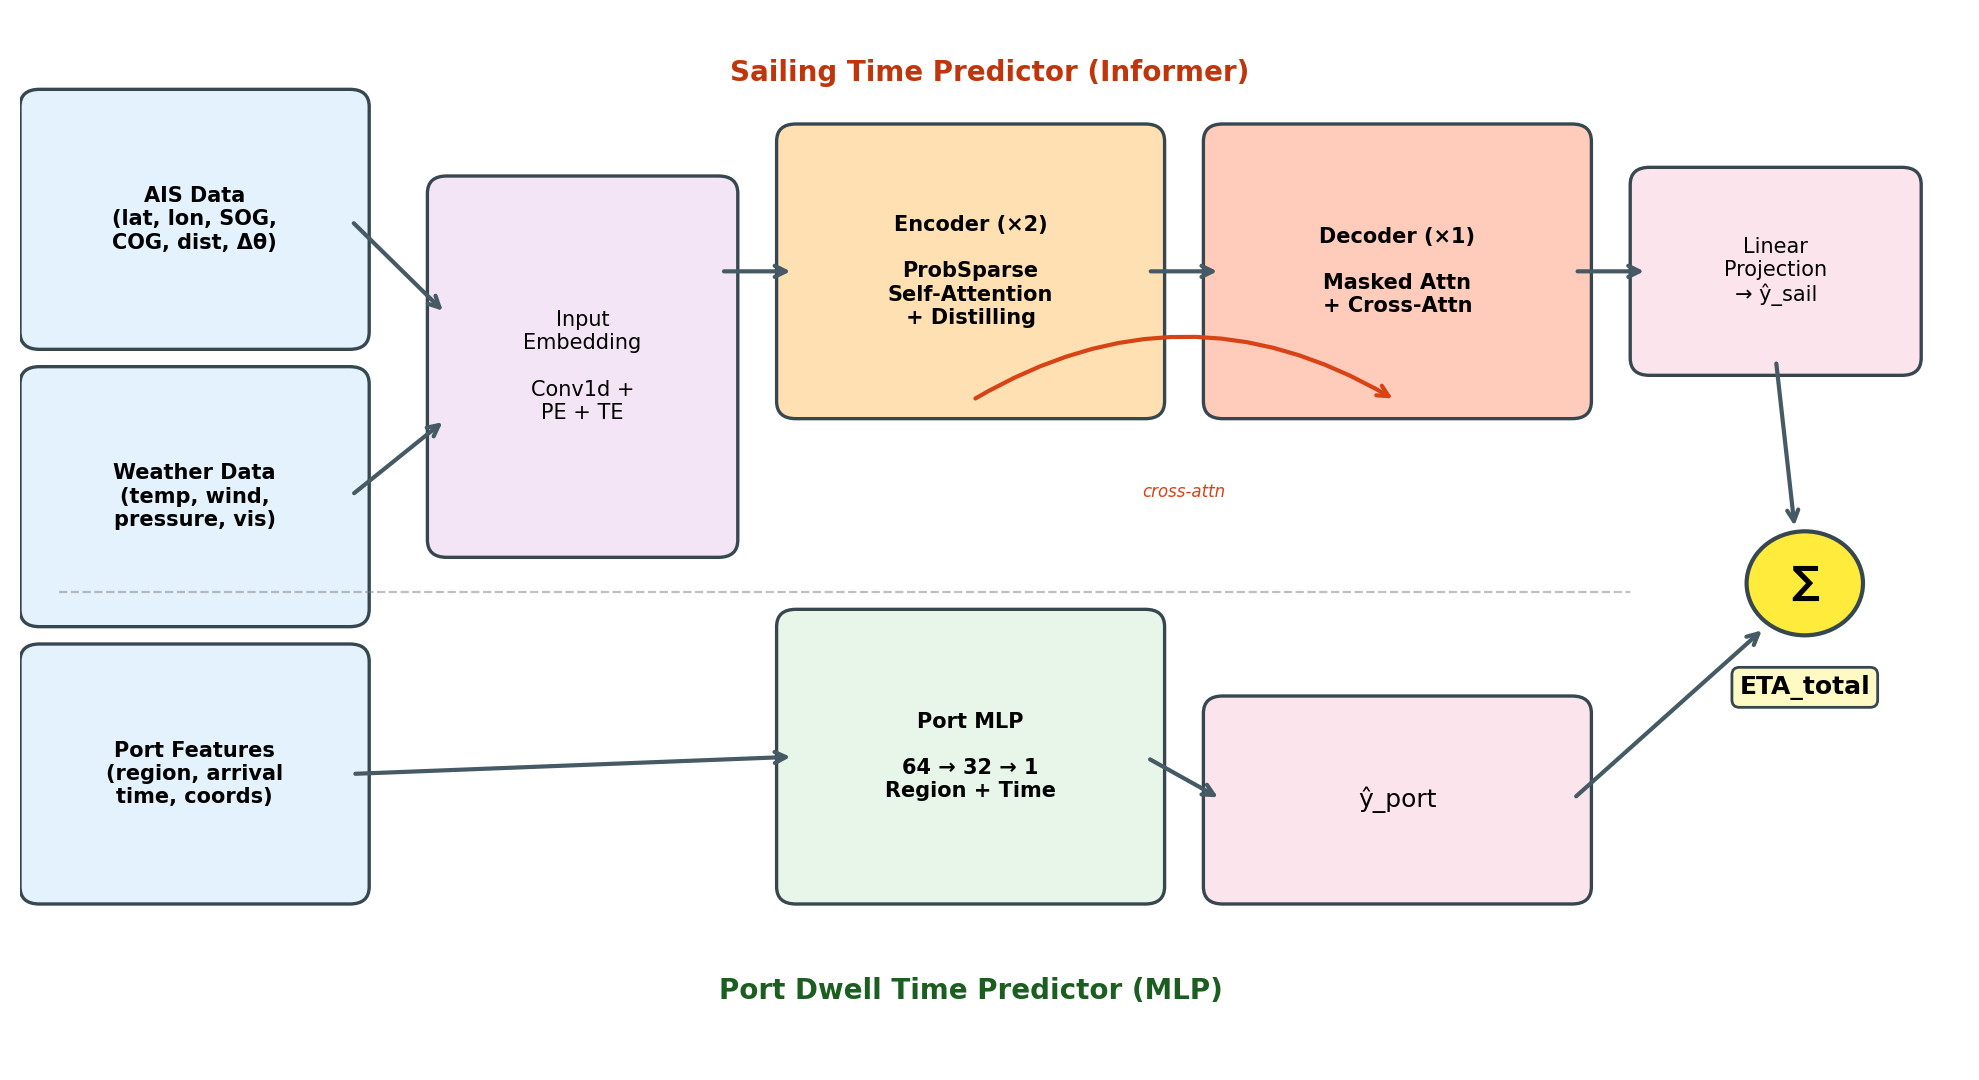
\includegraphics[width=\columnwidth]{architecture.pdf}
    \caption{Overview of the decoupled ETA prediction architecture. A candidate model predicts sailing time from AIS sequences enriched with weather features, while a separate MLP estimates port-dwell time. The final ETA is the sum of both predictions.}
    \label{fig:architecture}
\end{figure}

\subsection{Input Representation}

Each input sequence consists of $L_{\text{enc}} = 48$ consecutive AIS observations.
At each time step $t$, the feature vector $x_t \in \mathbb{R}^{11}$ comprises:

\begin{itemize}
    \item \textbf{Navigation features} ($d_{\text{nav}} = 6$): latitude, longitude, speed over ground (SOG), course over ground (COG), great-circle distance to destination ($\text{dist\_km}$), and bearing difference ($\Delta\theta$) between COG and the bearing toward the destination.
    \item \textbf{Meteorological features} ($d_{\text{wx}} = 5$): temperature, wind speed, wind level, mean sea-level pressure (PRMSL), and visibility.
\end{itemize}

The distance to destination and bearing difference are computed using the Haversine formula:
\begin{equation}
    d = 2R \arcsin\!\left(\sqrt{\sin^2\!\frac{\Delta\phi}{2} + \cos\phi_1 \cos\phi_2 \sin^2\!\frac{\Delta\lambda}{2}}\right)
    \label{eq:haversine}
\end{equation}
where $R = 6{,}371$ km is the Earth's radius, $\phi$ denotes latitude, and $\lambda$ denotes longitude.

Navigation features undergo min-max normalization to $[0, 1]$ with clipping at $[-0.5, 1.5]$ to handle out-of-distribution test samples.
The target variable (remaining hours) is transformed via log-standardization: $\tilde{y} = (\ln(1+y) - \mu) / \sigma$, where $\mu$ and $\sigma$ are computed from the training set.

\subsection{Voyage Extraction and Port-Stop Detection}
\label{sec:voyage_extraction}

Extracting individual voyages from the continuous AIS stream is a critical preprocessing step.
We employ a speed-based segmentation approach with the following criteria:

\begin{enumerate}
    \item \textbf{Stop detection}: A vessel is classified as \textit{stopped} when its SOG falls below $\tau_{\text{stop}} = 0.3$~knots. The binary stop indicator $s_t = \mathbb{1}[\text{SOG}_t < \tau_{\text{stop}}]$ is computed for each AIS record. Consecutive records with the same stop state are grouped into segments via cumulative sum of state changes.
    \item \textbf{Stop validation}: A stopped segment is considered a valid \textit{port stop} only if its duration exceeds $T_{\text{min\_stop}} = 2$~hours, filtering out brief anchorages and speed measurement noise.
    \item \textbf{Sailing segment filtering}: Sailing segments between successive port stops are retained only if they satisfy: duration $\geq T_{\text{min\_sail}} = 6$~hours and number of AIS records $\geq N_{\text{min}} = 50$. This eliminates short harbor maneuvers and data-sparse segments.
    \item \textbf{Trans-Pacific filtering}: To focus on the target route, we retain only voyages connecting Asian ports (longitude $> 100^\circ$E or $< 150^\circ$W) to U.S.\ West Coast ports ($-130^\circ < \text{lon} < -115^\circ$), identified by the geographic coordinates of voyage endpoints.
    \item \textbf{Duration filtering}: Voyages exceeding 720 hours (30 days) are excluded as likely erroneous or multi-stop itineraries.
\end{enumerate}

This pipeline yields 9,087 valid voyages from 3,940 unique vessels.

\subsection{Model Selection Rationale}
\label{sec:model_selection}

Following the architectural taxonomy proposed by recent deep time-series forecasting surveys~\cite{kim2025comprehensive, zeng2023transformers}, we select ten models covering five major families to ensure a comprehensive and systematic comparison:

\begin{enumerate}
    \item \textbf{Recurrent models} capture sequential dependencies through hidden state propagation. We include \textit{LSTM}~\cite{hochreiter1997lstm} and \textit{GRU}~\cite{cho2014gru}, the two most widely adopted variants, to evaluate whether gating mechanisms provide meaningful advantages.

    \item \textbf{Convolutional models} extract local temporal patterns through learnable filters. We include \textit{1D-CNN} (standard multi-layer convolutional network) and \textit{TCN}~\cite{bai2018tcn} (dilated causal convolutions with exponentially growing receptive fields), representing the two dominant convolutional paradigms.

    \item \textbf{Attention-based models} use self-attention to capture long-range dependencies. We include a \textit{Vanilla Transformer}~\cite{vaswani2017attention} (encoder-only with average pooling), a \textit{Conv-Transformer} hybrid (CNN feature extraction followed by Transformer encoding), and the \textit{Informer}~\cite{zhou2021informer} (ProbSparse attention with distilling). This family receives the most representatives given its recent prominence in the literature.

    \item \textbf{Tree-based models} operate on tabular feature representations. We include \textit{XGBoost}~\cite{chen2016xgboost}, the dominant gradient-boosted tree method, which requires hand-crafted statistical features extracted from the 48-step input window (last-step values, means, standard deviations, and deltas).

    \item \textbf{Feedforward models} serve as non-sequential baselines. We include a \textit{multi-layer perceptron (MLP)} operating on flattened input vectors, and \textit{Ridge Regression} ($L_2$-regularized linear regression on summary statistics) as the simplest baseline.
\end{enumerate}

\subsection{Model Configurations}

Table~\ref{tab:model_configs} summarizes the configuration and parameter counts for all models.
All neural models use the same input representation (48$\times$11 feature sequences) except XGBoost and Ridge, which operate on hand-crafted tabular features.

\begin{table}[t]
    \centering
    \caption{Model Configurations and Parameter Counts}
    \label{tab:model_configs}
    \begin{tabular}{llr}
        \toprule
        \textbf{Model} & \textbf{Key Configuration} & \textbf{Params} \\
        \midrule
        Ridge & $L_2$ regularization & -- \\
        MLP & $512{\to}256{\to}128$, BN, dropout & 270K \\
        XGBoost & 500 rounds, GPU hist & -- \\
        \midrule
        LSTM & 2 layers, $h{=}256$ & 802K \\
        GRU & 2 layers, $h{=}256$ & 610K \\
        \midrule
        1D-CNN & 3 Conv1d, MaxPool, AvgPool & 350K \\
        TCN & 4 dilated blocks $[128,128,256,256]$ & 600K \\
        \midrule
        Transformer & 3 enc layers, $d{=}256$, 8 heads & 1.6M \\
        Conv-Trans. & 2 Conv1d $+$ 2 enc layers, $d{=}256$ & 1.5M \\
        Informer & 2 enc $+$ 1 dec, $d{=}512$, ProbSparse & 11.3M \\
        \bottomrule
    \end{tabular}
\end{table}

\subsubsection{Informer Architecture Details}

Among the evaluated models, the Informer~\cite{zhou2021informer} has the most complex architecture.
Its key innovations include:
(1) ProbSparse self-attention, which identifies the most informative queries through a KL-divergence-based sparsity measure, reducing attention complexity to $O(L \log L)$;
(2) self-attention distilling, which progressively halves the sequence length through Conv1d + MaxPool operations between encoder layers;
and (3) a generative-style decoder that produces predictions in a single forward pass.

The input embedding combines three components:
\begin{equation}
    \mathbf{X}_{\text{feed}}^{(t)} = \alpha \, \mathbf{u}_t + \text{PE}_{t} + \sum_{p} \text{SE}_{t}^{(p)}
    \label{eq:embedding}
\end{equation}
where $\mathbf{u}_t$ is the scalar projection of raw features through a 1D convolution ($d \to d_{\text{model}}$); $\text{PE}_{t}$ is fixed sinusoidal positional encoding; and $\text{SE}_{t}^{(p)}$ are learnable temporal embeddings for each granularity $p \in \{\text{minute, hour, weekday, day, month}\}$.

\subsection{Port Dwell Time Predictor}

The port-dwell-time predictor is a two-layer MLP ($64 \to 32 \to 1$) with ReLU activation, batch normalization, and 20\% dropout.
It takes as input the destination port region (one-hot encoded among six predefined regions), arrival coordinates, and cyclically encoded temporal features (month and weekday as sine/cosine pairs).
This model is shared across all sailing-time predictors and is not part of the architecture comparison.


%==============================================================
\section{Experiments}
%==============================================================

\subsection{Dataset}

We use a proprietary AIS dataset covering trans-Pacific shipping routes between Chinese ports and the U.S.\ West Coast, spanning from January 2021 to March 2025.
The raw dataset contains approximately 35.9 million AIS position reports from 3,940 unique vessels.

Each AIS record includes the Maritime Mobile Service Identity (MMSI), timestamp, longitude, latitude, speed over ground (SOG, in knots), and course over ground (COG, in degrees).
Meteorological observations---temperature, wind speed, wind level (Beaufort scale), mean sea-level pressure, and horizontal visibility---are matched to each AIS record from contemporary weather data sources.

Individual voyages are extracted using the speed-based segmentation procedure described in Section~\ref{sec:voyage_extraction}.
After filtering, the dataset is partitioned by voyage into 70\% training, 15\% validation, and 15\% test splits, resulting in approximately 13.1 million training sequences, 2.9 million validation sequences, and 2.9 million test sequences.
Table~\ref{tab:dataset} summarizes the dataset statistics.

\begin{table}[t]
    \centering
    \caption{Dataset Statistics}
    \label{tab:dataset}
    \begin{tabular}{lc}
        \toprule
        \textbf{Statistic} & \textbf{Value} \\
        \midrule
        Total AIS records & 35,866,596 \\
        Unique vessels (MMSI) & 3,940 \\
        Extracted voyages & 9,087 \\
        Voyage duration range & $6$--$720$ hours \\
        \midrule
        Training sequences & 13,126,450 \\
        Validation sequences & 2,876,287 \\
        Test sequences & 2,859,888 \\
        \midrule
        Navigation features & 6 \\
        Weather features & 5 \\
        Total input dimensions & 11 \\
        Sequence length & 48 \\
        \bottomrule
    \end{tabular}
\end{table}


\subsection{Experimental Protocol}

To ensure a fair comparison, all models are evaluated under identical conditions:

\begin{itemize}
    \item \textbf{Data}: Same train/val/test splits (70/15/15\% by voyage), same 11-dimensional feature set, and same min-max normalization with log-standardized targets.
    \item \textbf{Loss}: Huber loss ($\delta = 1.0$) for all models.
    \item \textbf{Optimizer}: Adam ($\text{lr} = 10^{-3}$) for all neural models; the Informer uses $\text{lr} = 4 \times 10^{-4}$ with ReduceLROnPlateau scheduling per its original training recipe.
    \item \textbf{Early stopping}: Patience of 3 epochs on validation loss for all neural models.
    \item \textbf{Batch size}: 4,096 for all models.
    \item \textbf{Hardware}: Single NVIDIA RTX PRO 6000 GPU (96\,GB VRAM). XGBoost uses GPU-accelerated histogram building.
\end{itemize}

Data loading employs memory-mapped arrays (NumPy memmap) to handle the 13M+ training sequences without exceeding system memory, with 64 data loader workers and pinned GPU memory transfers.


\subsection{Evaluation Metrics}

We report the following metrics on the test set:

\begin{itemize}
    \item \textbf{MAE} (Mean Absolute Error, in hours): $\frac{1}{N}\sum_{i}|\hat{y}_i - y_i|$
    \item \textbf{RMSE} (Root Mean Squared Error, in hours): $\sqrt{\frac{1}{N}\sum_{i}(\hat{y}_i - y_i)^2}$
    \item \textbf{MAPE} (Mean Absolute Percentage Error, \%): computed only on samples where $y_i > 24$ hours, to avoid division-by-zero artifacts on near-arrival predictions.
\end{itemize}


\subsection{Main Results}

Table~\ref{tab:main_results} presents the comparison of all ten methods on the test set.
Fig.~\ref{fig:baseline_comparison} provides a visual comparison.

\begin{table}[t]
    \centering
    \caption{Comparison of ETA Prediction Methods on Test Set. All models use standard Huber loss. Best results in \textbf{bold}, second-best \underline{underlined}.}
    \label{tab:main_results}
    \begin{tabular}{llccc}
        \toprule
        \textbf{Family} & \textbf{Method} & \textbf{MAE (h)} & \textbf{RMSE (h)} & \textbf{MAPE (\%)} \\
        \midrule
        \multirow{2}{*}{Feedforward} & Ridge & 58.30 & 367.19 & 29.35 \\
        & MLP & \underline{15.73} & \underline{26.80} & 9.67 \\
        \midrule
        \multirow{2}{*}{Recurrent} & LSTM & 15.79 & 27.40 & \underline{9.43} \\
        & GRU & 16.03 & 27.28 & 9.62 \\
        \midrule
        \multirow{2}{*}{Convolutional} & 1D-CNN & 16.08 & 27.53 & 9.90 \\
        & TCN & 17.19 & 28.13 & 10.95 \\
        \midrule
        Tree & XGBoost & \textbf{15.14} & \textbf{26.05} & \textbf{9.33} \\
        \midrule
        \multirow{3}{*}{Attention} & Transformer & 18.12 & 29.78 & 10.67 \\
        & Conv-Trans. & 16.60 & 27.52 & 10.07 \\
        & Informer & 16.20 & 27.26 & 10.53 \\
        \bottomrule
    \end{tabular}
\end{table}

\begin{figure}[t]
    \centering
    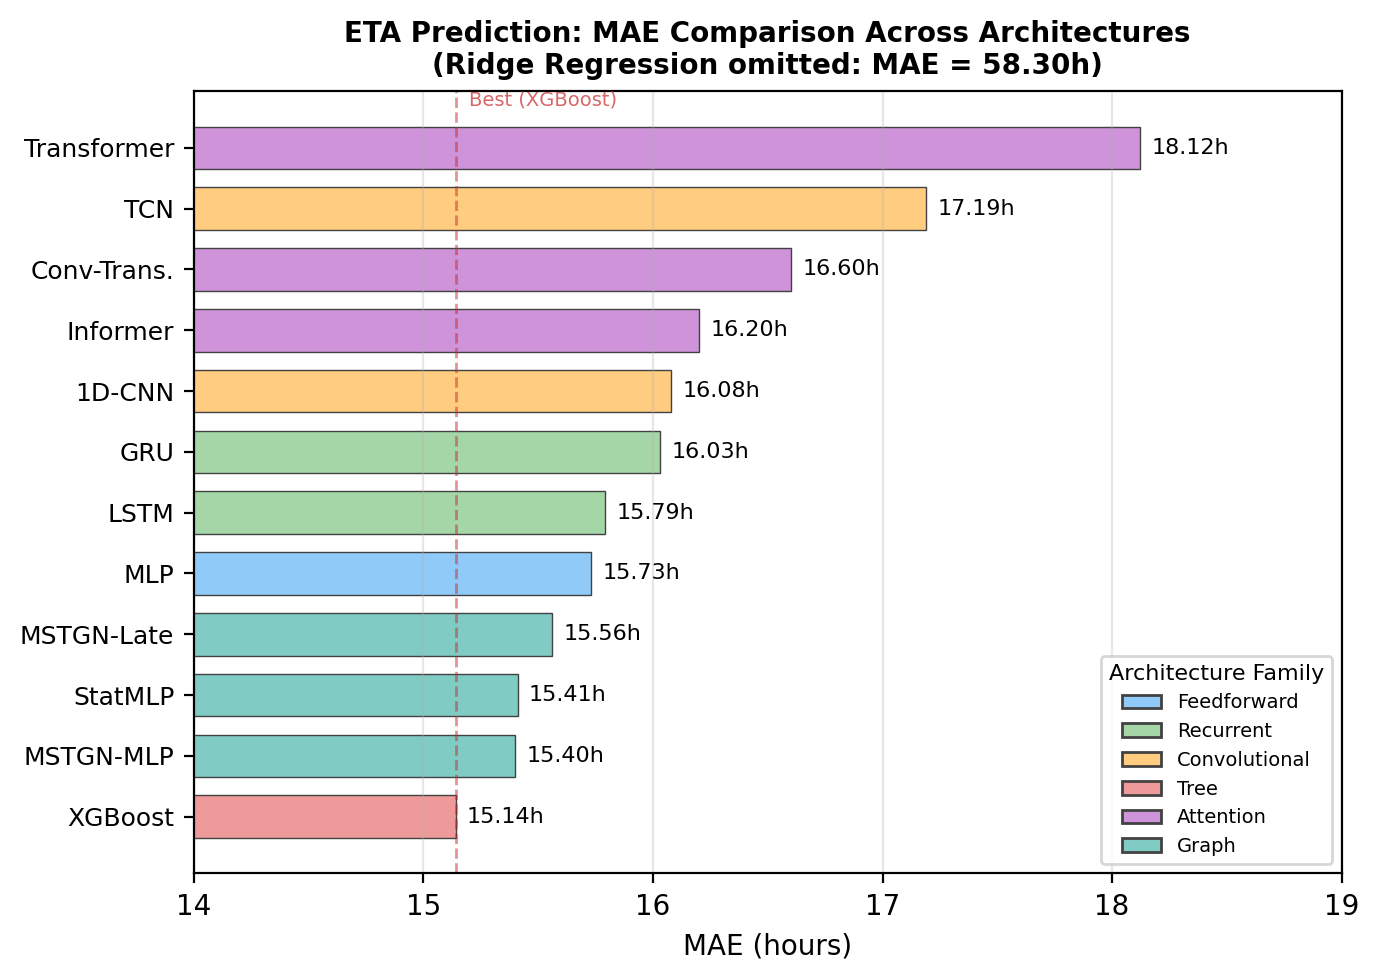
\includegraphics[width=\columnwidth]{baseline_comparison.pdf}
    \caption{MAE comparison across all ten methods, grouped by architectural family. Ridge Regression (58.30\,h) is omitted for visual clarity. The dashed line indicates the best result (XGBoost, 15.14\,h). Attention-based models (Transformer, Conv-Trans., Informer) consistently underperform simpler alternatives.}
    \label{fig:baseline_comparison}
\end{figure}

\subsubsection{Key Findings}

\paragraph{Finding 1: XGBoost achieves the best overall performance.}
XGBoost achieves the lowest MAE (15.14\,h), RMSE (26.05\,h), and MAPE (9.33\%), outperforming all neural sequence models despite operating on hand-crafted statistical features rather than raw sequential input.
This result aligns with recent findings in time-series forecasting~\cite{zeng2023transformers} that simpler models can rival or surpass attention-based architectures, particularly when strong engineered features are available.

\paragraph{Finding 2: Feature engineering dominates architecture choice.}
Excluding Ridge, all models achieve MAEs within a 15.14--18.12\,h range.
The top five models (XGBoost, MLP, LSTM, GRU, 1D-CNN) cluster within 15.14--16.08\,h (${<}7\%$ relative spread), despite spanning four distinct architectural families and parameter counts from 270K to 11.3M.
The highly predictive \textit{distance-to-destination} feature provides a strong prior on remaining time, reducing the marginal benefit of sophisticated temporal modeling.

\paragraph{Finding 3: Attention-based models do not justify their complexity.}
The Vanilla Transformer (18.12\,h MAE, 1.6M params) performs worst among the neural models.
The Informer (16.20\,h, 11.3M params) and Conv-Transformer (16.60\,h, 1.2M params) fare better but still lag behind the simpler MLP (15.73\,h, 270K params).
These architectures, designed for long-horizon multi-step forecasting, appear unnecessary for the single-step prediction task considered here ($L_{\text{pred}} = 1$).

\paragraph{Finding 4: Convolutional models show mixed results.}
The 1D-CNN (16.08\,h) approaches the MLP and recurrent models, but the TCN (17.19\,h) underperforms, possibly due to overfitting with its dilated convolutions on a relatively short 48-step input.
The TCN's exponentially growing receptive field may be more beneficial for longer sequences than the ones considered here.


\subsection{Ablation Studies}

\subsubsection{Effect of Weather Features}

To quantify the contribution of meteorological features, we train the Informer model with identical hyperparameters using only the six navigation features ($d = 6$) versus the full 11-dimensional input ($d = 11$).
As shown in Table~\ref{tab:ablation_weather}, incorporating weather features reduces MAE from 17.43 hours to 16.20 hours, a 7.1\% relative improvement.
This confirms that en-route weather conditions provide complementary information beyond what navigation features alone capture.

\begin{table}[t]
    \centering
    \caption{Ablation: Effect of Weather Features (Informer)}
    \label{tab:ablation_weather}
    \begin{tabular}{lccc}
        \toprule
        \textbf{Features} & \textbf{MAE (h)} & $\Delta$\textbf{MAE (h)} & $\Delta$\textbf{MAE (\%)} \\
        \midrule
        Navigation only ($d=6$) & 17.43 & -- & -- \\
        Navigation + Weather ($d=11$) & \textbf{16.20} & $-1.23$ & $-7.1\%$ \\
        \bottomrule
    \end{tabular}
\end{table}

\subsubsection{Effect of Asymmetric Loss (Negative Result)}
\label{sec:ablation_loss}

In maritime logistics, underestimating the arrival time is typically more costly than overestimating it, as it can lead to missed berth windows, idle cranes, and cascading schedule disruptions.
Motivated by this asymmetry, we investigate an \textit{Asymmetric Huber Loss} that penalizes underestimation by a factor of $\alpha$ and optionally upweights long-haul voyages by a factor proportional to the target value:
\begin{equation}
    \mathcal{L} = \frac{1}{N} \sum_{i=1}^{N} w_{\text{asym}}^{(i)} \cdot w_{\text{target}}^{(i)} \cdot \mathcal{H}_\delta(e_i)
    \label{eq:loss}
\end{equation}
where $w_{\text{asym}} = \alpha$ if $e_i < 0$ (underestimation), else $1$; and $w_{\text{target}} = 1 + \beta \cdot \text{ReLU}(y_i)$.

We test two configurations: (A)~$\alpha{=}1.5, \beta{=}0.3$ and (B)~$\alpha{=}1.2, \beta{=}0$.
As shown in Table~\ref{tab:ablation_loss}, both configurations significantly degrade overall accuracy.
Configuration A increases MAE by 13.8\% (16.20 $\to$ 18.43\,h), while Configuration B increases MAE by 17.6\% (16.20 $\to$ 19.05\,h).

\begin{table}[t]
    \centering
    \caption{Ablation: Asymmetric Loss on Informer (Negative Result)}
    \label{tab:ablation_loss}
    \begin{tabular}{lccc}
        \toprule
        \textbf{Loss Configuration} & \textbf{MAE (h)} & \textbf{RMSE (h)} & \textbf{MAPE (\%)} \\
        \midrule
        Huber (symmetric) & \textbf{16.20} & \textbf{27.26} & 10.53 \\
        Asym. ($\alpha{=}1.5, \beta{=}0.3$) & 18.43 & 30.00 & 12.32 \\
        Asym. ($\alpha{=}1.2, \beta{=}0$) & 19.05 & 33.54 & \textbf{11.13} \\
        \bottomrule
    \end{tabular}
\end{table}

This negative result suggests that naive asymmetric loss application may cause the model to systematically overestimate, degrading calibration.
The asymmetric penalty distorts the loss landscape in ways that the optimizer cannot easily compensate for, particularly when combined with log-standardized targets and early stopping based on symmetric validation loss.
We report this finding to caution practitioners against applying asymmetric losses without careful calibration.


\subsubsection{Training Dynamics}

Fig.~\ref{fig:training_curve} shows the training and validation loss curves for the Informer.
The model achieves its best validation loss at epoch 2 (val loss = 0.0194), after which validation loss begins to increase while training loss continues to decrease, indicating the onset of overfitting.
Early stopping triggers at epoch 5 (patience = 3).

\begin{figure}[t]
    \centering
    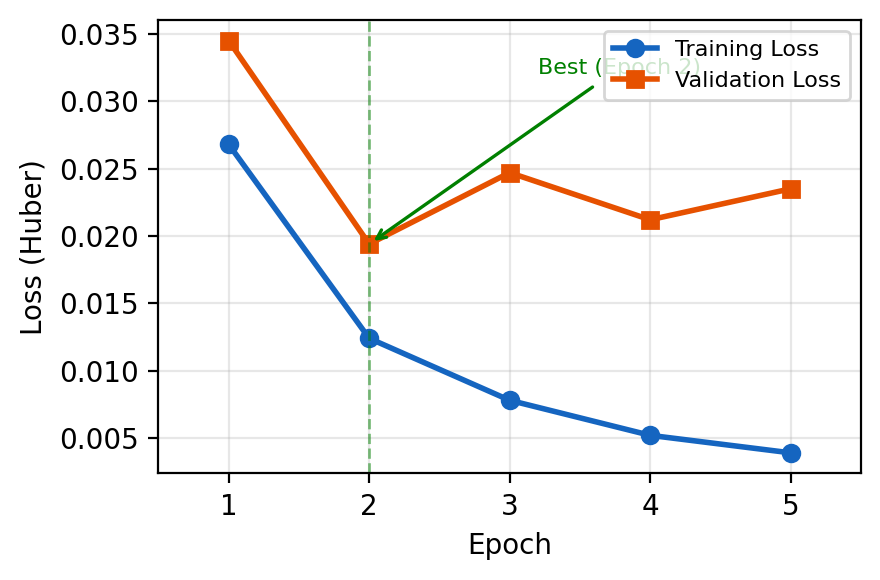
\includegraphics[width=0.85\columnwidth]{training_curve.pdf}
    \caption{Informer training and validation loss curves. The best model is selected at epoch 2; training beyond this point leads to overfitting.}
    \label{fig:training_curve}
\end{figure}


\subsection{Error Analysis}

To understand prediction failures, we analyze test samples where the absolute error exceeds 200 hours.
These ``bad cases'' predominantly involve:
(1) extremely long-haul voyages ($>500$ hours) where small relative errors translate to large absolute errors;
(2) voyages with anomalous speed profiles (e.g., prolonged slow steaming or mid-ocean stops);
and (3) voyages with missing or zero-valued weather features.

The MAE-by-sailing-day analysis reveals that prediction accuracy is highest during the first few days of a voyage and degrades for predictions made very early (when more uncertainty remains about the vessel's routing and speed profile).


%==============================================================
\section{Related Work}
%==============================================================

\paragraph{Vessel ETA Prediction.}
Machine learning approaches to vessel ETA prediction have evolved from traditional methods (SVR~\cite{liu2019svr}, Random Forest~\cite{zhang2019rf}) to deep learning architectures.
Zhang et al.~\cite{zhang2022lstm} applied LSTM-GAN to ship trajectory prediction, while Han et al.~\cite{han2021gru} proposed a GRU-based method for vessel trajectory forecasting.
Dong et al.~\cite{dong2023transformer} introduced a Transformer with position encoding attention for ship trajectory prediction.
El~Mekkaoui et al.~\cite{elmekkaoui2023} conducted a comprehensive study of deep learning approaches for vessel ETA at bulk ports.
Lloret-Batlle et al.~\cite{lloretbatlle2025} recently demonstrated ANN-based cross-Pacific vessel ETA prediction using AIS data, achieving MAE of 4 hours at 1,500 nautical miles from port.
However, most studies evaluate only one or two architectures, making cross-method comparisons difficult.

\paragraph{Time-Series Forecasting Benchmarks.}
The importance of fair benchmarking has been highlighted by Zeng et al.~\cite{zeng2023transformers}, who showed that simple linear models can outperform Transformers for long-horizon time-series forecasting.
Kim et al.~\cite{kim2025comprehensive} proposed a comprehensive taxonomy classifying deep time-series models into Transformer, CNN, RNN, MLP, SSM, and LLM families, and emphasized the need for standardized evaluation protocols.
Bai et al.~\cite{bai2018tcn} demonstrated that TCNs provide a strong alternative to recurrent architectures for sequence modeling.
Our work applies this benchmarking philosophy to the maritime ETA domain.


%==============================================================
\section{Conclusion}
%==============================================================

We presented a systematic empirical comparison of ten forecasting models from five architectural families for vessel ETA prediction on trans-Pacific routes.
Our evaluation, conducted on a large-scale AIS dataset with 35.9 million position reports under strictly controlled experimental conditions, reveals several findings of practical significance.

First, XGBoost achieves the best performance (MAE = 15.14\,h), outperforming all neural sequence models including the Informer despite its relative simplicity.
This suggests that for single-step ETA prediction with strong engineered features (particularly distance-to-destination), tree-based models remain highly competitive.

Second, incorporating meteorological features yields a consistent 7.1\% MAE improvement (17.43 $\to$ 16.20\,h), confirming that weather conditions provide complementary predictive signal beyond navigation features alone.

Third, asymmetric loss functions intended to reduce underestimation significantly degrade overall accuracy (up to 17.6\% MAE increase), cautioning against their naive application in this setting.

Finally, the narrow performance spread among the top neural models (15.73--16.20\,h MAE for MLP, LSTM, GRU, CNN, and Informer) suggests that the bottleneck in vessel ETA prediction lies in feature informativeness and data quality rather than model architecture.
These findings provide practical guidance for maritime stakeholders seeking to deploy ETA prediction systems.

Future work will explore ocean current data integration, multi-step prediction horizons (where attention mechanisms may provide greater benefit), and extending the evaluation to global shipping routes beyond the trans-Pacific corridor.


%==============================================================
% References
%==============================================================

\bibliographystyle{IEEEtran}

\begin{thebibliography}{99}

\bibitem{unctad2023}
UNCTAD, ``Review of Maritime Transport 2023,'' United Nations Conference on Trade and Development, 2023.

\bibitem{park2021}
K.~Park, J.~Kim, and Y.~Lee, ``Deep learning-based vessel arrival time prediction,'' \textit{J. Marine Sci. Engineering}, vol.~9, no.~10, p.~1107, 2021.

\bibitem{fang2022}
S.~Fang, R.~Zhu, and Y.~Xu, ``Vessel ETA prediction using AIS data and machine learning,'' \textit{Ocean Engineering}, vol.~261, p.~112079, 2022.

\bibitem{zhang2019rf}
Z.~Zhang, C.~Yin, and T.~Li, ``A random-forest-based model for ship destination prediction,'' \textit{ISPRS Int. J. Geo-Inf.}, vol.~8, no.~8, p.~367, 2019.

\bibitem{liu2019svr}
L.~Liu, Y.~Zhang, and Z.~Guo, ``Ship trajectory prediction based on SVR optimized by ACDE,'' \textit{J. Coastal Res.}, vol.~94, pp.~52--56, 2019.

\bibitem{zhang2022lstm}
D.~Zhang, J.~Zhang, and K.~Zhang, ``LSTM-GAN for ship trajectory prediction with varying time intervals,'' \textit{Ocean Engineering}, vol.~245, p.~110454, 2022.

\bibitem{han2021gru}
X.~Han, C.~Zheng, and J.~Guo, ``GRU-based vessel trajectory prediction method,'' \textit{J. Navigation}, vol.~74, no.~6, pp.~1308--1322, 2021.

\bibitem{dong2023transformer}
D.~Dong, W.~Li, and P.~Liu, ``Ship trajectory prediction based on Transformer with position encoding attention,'' \textit{Ocean Engineering}, vol.~272, p.~113859, 2023.

\bibitem{zhou2021informer}
H.~Zhou, S.~Zhang, J.~Peng, S.~Zhang, J.~Li, H.~Xiong, and W.~Zhang, ``Informer: Beyond efficient Transformer for long sequence time-series forecasting,'' in \textit{Proc. AAAI Conf. Artif. Intell.}, vol.~35, no.~12, pp.~11106--11115, 2021.

\bibitem{xiong2024informertp}
C.~Xiong, H.~Shi, J.~Li, X.~Wu, and R.~Gao, ``Informer-based model for long-term ship trajectory prediction,'' \textit{J. Marine Sci. Engineering}, vol.~12, no.~8, p.~1269, 2024.

\bibitem{kingma2015adam}
D.~P.~Kingma and J.~Ba, ``Adam: A method for stochastic optimization,'' in \textit{Proc. Int. Conf. Learn. Representations (ICLR)}, 2015.

\bibitem{hochreiter1997lstm}
S.~Hochreiter and J.~Schmidhuber, ``Long short-term memory,'' \textit{Neural Computation}, vol.~9, no.~8, pp.~1735--1780, 1997.

\bibitem{cho2014gru}
K.~Cho, B.~van Merri{\"e}nboer, C.~Gulcehre, D.~Bahdanau, F.~Bougares, H.~Schwenk, and Y.~Bengio, ``Learning phrase representations using RNN encoder-decoder for statistical machine translation,'' in \textit{Proc. EMNLP}, pp.~1724--1734, 2014.

\bibitem{chen2016xgboost}
T.~Chen and C.~Guestrin, ``XGBoost: A scalable tree boosting system,'' in \textit{Proc. ACM SIGKDD}, pp.~785--794, 2016.

\bibitem{vaswani2017attention}
A.~Vaswani, N.~Shazeer, N.~Parmar, J.~Uszkoreit, L.~Jones, A.~N.~Gomez, {\L}.~Kaiser, and I.~Polosukhin, ``Attention is all you need,'' in \textit{Advances in Neural Information Processing Systems}, vol.~30, 2017.

\bibitem{bai2018tcn}
S.~Bai, J.~Z.~Kolter, and V.~Koltun, ``An empirical evaluation of generic convolutional and recurrent networks for sequence modeling,'' \textit{arXiv preprint arXiv:1803.01271}, 2018.

\bibitem{zeng2023transformers}
A.~Zeng, M.~Chen, L.~Zhang, and Q.~Xu, ``Are Transformers effective for time series forecasting?'' in \textit{Proc. AAAI Conf. Artif. Intell.}, vol.~37, no.~9, pp.~11121--11128, 2023.

\bibitem{kim2025comprehensive}
J.~Kim, H.~Lee, and S.~Park, ``Deep time series forecasting models: A comprehensive survey,'' \textit{Mathematics}, vol.~12, no.~10, p.~1504, 2024.

\bibitem{elmekkaoui2023}
S.~El~Mekkaoui, L.~Benabbou, and A.~Berrado, ``Deep learning models for vessel estimated time of arrival: A case study of bulk port operations,'' \textit{J. Marine Sci. Engineering}, vol.~11, no.~6, p.~1230, 2023.

\bibitem{lloretbatlle2025}
R.~Lloret-Batlle, R.~Mounce, and J.~Sherwood, ``Cross-Pacific vessel estimated time of arrival prediction with AIS trajectory data,'' \textit{Maritime Transport Research}, vol.~7, p.~100108, 2025.

\end{thebibliography}

\end{document}
